\documentclass{beamer}
\usetheme{ODK}
\usepackage{tikz}

\usepackage[utf8]{inputenc}
\usepackage{eurosym}
\usepackage{graphicx}
\graphicspath{{../../../../Proposal/Pictures/}}

\makeatletter
\newskip\@bigflushglue \@bigflushglue = -100pt plus 1fil
\def\bigcenter{\trivlist \bigcentering\item\relax}
\def\bigcentering{\let\\\@centercr\rightskip\@bigflushglue%
\leftskip\@bigflushglue
\parindent\z@\parfillskip\z@skip}
\def\endbigcenter{\endtrivlist}
\makeatother

\newcommand{\fr}[1]{}
\newcommand{\en}[1]{#1}
\newcommand{\blue}

\author{Nicolas M. Thiéry}
\title{Word of welcome}

\begin{document}

\begin{frame}
  \titlepage
\end{frame}

\begin{frame}{ODK's interviews}
  \url{https://opendreamkit.org/}
\end{frame}

\begin{frame}{ODK's use cases}
  \url{https://opendreamkit.org/tag/use-case}
\end{frame}

\begin{frame}{Aims}
  \begin{description}
  \item[Aim 1] Improve the productivity of researchers in pure mathematics and
    applications by further promoting collaborations on \textbf{Data},
    \textbf{Knowledge}, and \textbf{Software}
  \item[Aim 2] Make it easy for teams of researchers of any size to set up
    custom, collaborative \textbf{Virtual Research Environments}
    tailored to their specific needs, resources and workflows
  \item[Aim 3] Support the entire life-cycle of computational work in
    mathematical research, from \textbf{initial exploration} to
    \textbf{publication}, \textbf{teaching}, and \textbf{outreach}
  \item[Aim 4]  Maximise sustainability and impact in mathematics,
    neighbouring fields, and scientific computing.
  \end{description}
\end{frame}


\begin{frame}{OpenDreamKit's proposal}\label{our-proposal}
  \begin{itemize}
  \item Deliver a \textbf{VRE Toolkit for Mathematics}
  \item From the ecosystem of open source software for mathematics
  \item And the Jupyter interactive computing environment
  \end{itemize}
\end{frame}

\begin{frame}{OpenDreamKit's proposal}\label{our-proposal}
  \centerline{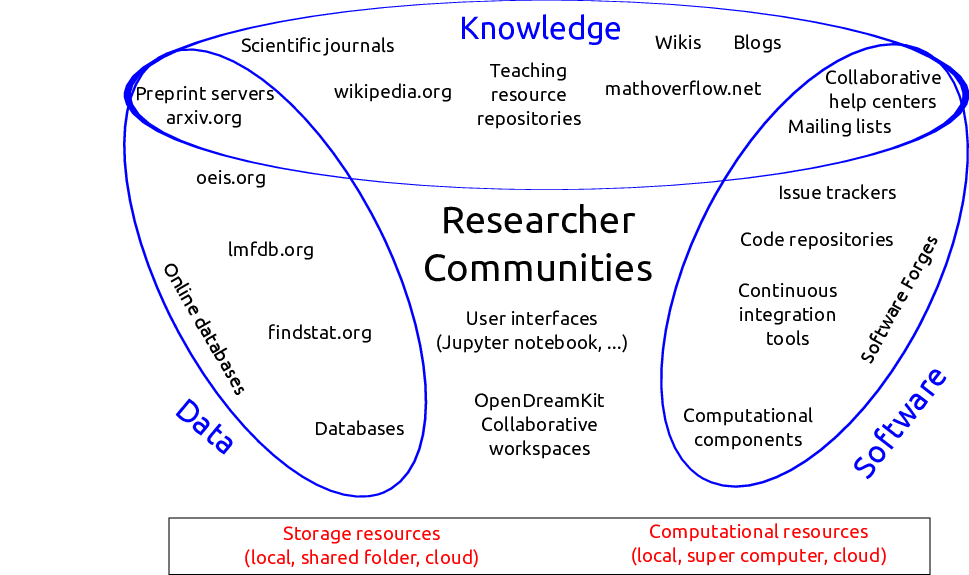
\includegraphics[height=.85\textheight]{TheBigPicture.pdf}}
\end{frame}

\begin{frame}[fragile]{A specific challenge: a rich variety of objects}
  \pause
  \blue{\fr{Nombres}\en{Numbers}:}\quad $42$, $\frac79$, $\frac{I+sqrt(3)}2$, $\pi$, $2.71828182845904523536028747?$
  \bigskip\pause

  \blue{Matrices:}
  $\left(\begin{array}{rrrr}
      4 & -1 & 1 & -1 \\
      -1 & 2 & -1 & -1 \\
      0 & 5 & 1 & 3
    \end{array}\right)$,
  $\left(\begin{array}{rrr}
      1.000 & 0.500 & 0.333 \\
      0.500 & 0.333 & 0.250 \\
      0.333 & 0.250 & 0.200
    \end{array}\right)$

  \bigskip\pause

  \blue{\fr{Polynômes}\en{Polynomials}:}\quad $-9x^{8} + x^{7} + x^{6} - 13x^{5} - x^{3} - 3x^{2} - 8x + 4$ %\sage{ZZ[x].random_element(degree=8)}$
  \bigskip\pause

  \blue{\fr{Séries}\en{Series}:}\quad $1 + 1 x + \frac{1}{2} x^{2} + \frac{1}{6} x^{3} + \frac{1}{24} x^{4} + \frac{1}{120} x^{5} + \cdots$
  % \sage{exp(x).series(x,6)}$
  \bigskip\pause

  \blue{\fr{Expressions symboliques, équations}\en{Symbolic expressions, equations}:}\quad $cos(x)^2 + sin(x)^2 == 1$

  \bigskip\pause

  \blue{\fr{Corps finis, extensions algébriques, courbes elliptiques, ...}
  \en{Finite fields, algebraic extensions, elliptic curves, ...}}

\end{frame}

\def\lr#1{\multicolumn{1}{|@{\hspace{.6ex}}c@{\hspace{.6ex}}|}{\raisebox{-.3ex}{$#1$}}}
\begin{frame}[fragile]{\fr{Objets combinatoires}\en{Combinatorial objects}}
  \begin{bigcenter}

    \raisebox{2ex}{$\begin{array}[b]{*{4}c}\cline{1-4}
        \lr{1}&\lr{3}&\lr{4}&\lr{7}\\\cline{1-4}
        \lr{2}&\lr{5}&\lr{6}\\\cline{1-3}
        \lr{8}\\\cline{1-1}
      \end{array}$}
    \qquad
    \scalebox{.7}{{\setlength\unitlength{4mm}
\begin{picture}(20,8)
\put(1,4){\circle*{0.5}}
\put(1.3,3.7){$\scriptstyle 1$}\put(2,3){\circle*{0.5}}
\put(2.3,2.7){$\scriptstyle 2$}\put(3,2){\circle*{0.5}}
\put(3.3,1.7){$\scriptstyle 3$}\put(2,3){\line(1,-1){1}}
\put(1,4){\line(1,-1){1}}
\put(4,5){\circle*{0.5}}
\put(4.3,4.7){$\scriptstyle 4$}\put(5,4){\circle*{0.5}}
\put(5.3,3.7){$\scriptstyle 5$}\put(6,1){\circle*{0.5}}
\put(6.3,0.7){$\scriptstyle 6$}\put(7,2){\circle*{0.5}}
\put(7.3,1.7){$\scriptstyle 7$}\put(8,1){\circle*{0.5}}
\put(8.3,0.7){$\scriptstyle 8$}\put(7,2){\line(-1,-1){1}}
\put(7,2){\line(1,-1){1}}
\put(9,3){\circle*{0.5}}
\put(9.3,2.7){$\scriptstyle 9$}\put(9,3){\line(-2,-1){2}}
\put(5,4){\line(4,-1){4}}
\put(4,5){\line(-3,-1){3}}
\put(4,5){\line(1,-1){1}}
\put(10,6){\circle*{0.5}}
\put(10.3,5.7){$\scriptstyle 10$}\put(11,5){\circle*{0.5}}
\put(11.3,4.7){$\scriptstyle 11$}\put(12,3){\circle*{0.5}}
\put(12.3,2.7){$\scriptstyle 12$}\put(13,4){\circle*{0.5}}
\put(13.3,3.7){$\scriptstyle 13$}\put(13,4){\line(-1,-1){1}}
\put(11,5){\line(2,-1){2}}
\put(10,6){\line(-6,-1){6}}
\put(10,6){\line(1,-1){1}}
\put(14,7){\circle*{0.5}}
\put(14.3,6.7){$\scriptstyle 14$}\put(15,5){\circle*{0.5}}
\put(15.3,4.7){$\scriptstyle 15$}\put(16,6){\circle*{0.5}}
\put(16.3,5.7){$\scriptstyle 16$}\put(17,4){\circle*{0.5}}
\put(17.3,3.7){$\scriptstyle 17$}\put(18,5){\circle*{0.5}}
\put(18.3,4.7){$\scriptstyle 18$}\put(18,5){\line(-1,-1){1}}
\put(16,6){\line(-1,-1){1}}
\put(16,6){\line(2,-1){2}}
\put(14,7){\line(-4,-1){4}}
\put(14,7){\line(2,-1){2}}
\put(14,7){\circle*{0.7}}
\end{picture}}
}
  \bigskip

  %\sage{DyckWord([1, 1, 1, 0, 0, 1, 0, 1, 0, 1, 1, 1, 0, 0, 0, 0, 1, 0, 1, 0])}$
  \scalebox{.3}{\hbox{$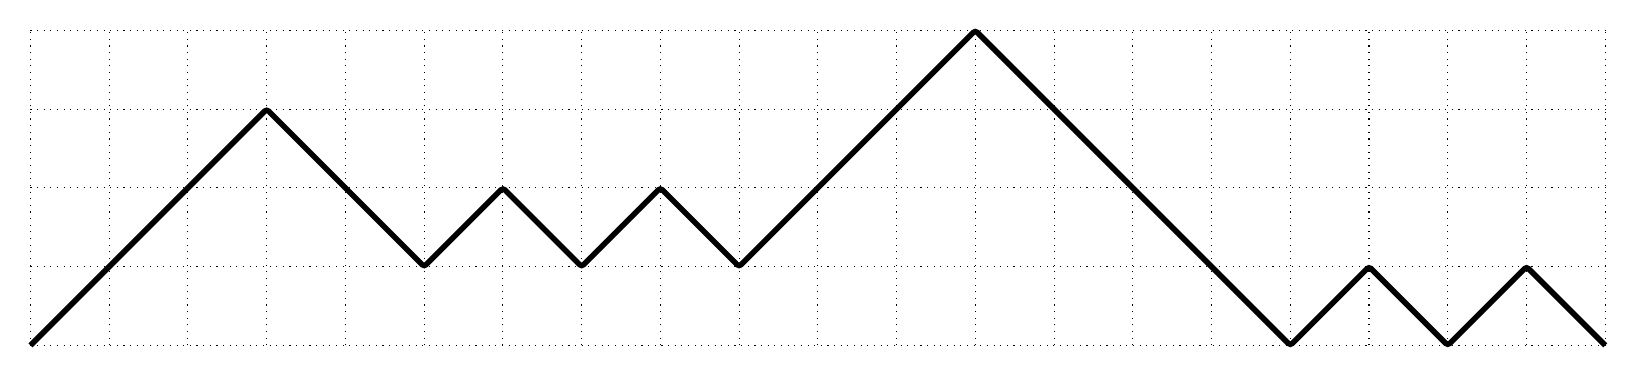
\begin{tikzpicture}[scale=1]
  \draw[dotted] (0, 0) grid (20, 4);
  \draw[rounded corners=1, color=black, line width=2] (0, 0) -- (1, 1) -- (2, 2) -- (3, 3) -- (4, 2) -- (5, 1) -- (6, 2) -- (7, 1) -- (8, 2) -- (9, 1) -- (10, 2) -- (11, 3) -- (12, 4) -- (13, 3) -- (14, 2) -- (15, 1) -- (16, 0) -- (17, 1) -- (18, 0) -- (19, 1) -- (20, 0);
\end{tikzpicture}$}}
  \bigskip

  $0100101001001010010100100101001001010010\cdots$
  \bigskip

  \tikzset{baseline=(current bounding box.east)}
\tikzset{level distance = 0.7cm}
\tikzset{level/.style={sibling distance = 3cm/(2+#1)}}
\tikzset{binnode/.style={draw, circle, inner sep=1.2pt, minimum width=1.2em,
                       fill=blue!10, rounded corners}}
$\scriptstyle\scriptsize
\frac{\frac{1}{6} q^{2} - \frac{1}{6} q}{q^{5}
      + 2 q^{4} + 3 q^{3} + 3 q^{2} + 2 q + 1}{
    \newcommand{\nodea}{\node [binnode] (a) {$a$}
      ;}\newcommand{\nodeb}{\node [binnode] (b) {$b$}
      ;}\newcommand{\nodec}{\node [binnode] (c) {$c$}
      ;}\newcommand{\noded}{\node [binnode] (d) {$d$}
      ;}\scalebox{.6}{\begin{tikzpicture}[auto] \matrix[column sep=.3cm, row
      sep=.3cm,ampersand replacement=\&]{
        \& \nodea  \&         \\
        \nodeb  \& \nodec  \& \noded  \\
      };

      \path[ultra thick] (a) edge (b) edge (c) edge (d);
    \end{tikzpicture}}} + \frac{q^{2}}{q^{5} + 2 q^{4} + 3 q^{3} + 3
      q^{2} + 2 q + 1}{ \newcommand{\nodea}{\node [binnode] (a)
      {$a$} ;}\newcommand{\nodeb}{\node [binnode] (b) {$b$}
      ;}\newcommand{\nodec}{\node [binnode] (c) {$c$}
      ;}\newcommand{\noded}{\node [binnode] (d) {$d$}
      ;}\scalebox{.6}{\begin{tikzpicture}[auto] \matrix[column sep=.3cm, row
      sep=.3cm,ampersand replacement=\&]{
        \& \nodea  \&         \\
        \nodeb  \&         \& \nodec  \\
        \&         \& \noded  \\
      };

      \path[ultra thick] (c) edge (d) (a) edge (b) edge (c);
    \end{tikzpicture}}} + \frac{\frac{1}{2} q}{q^{4} + q^{3} + 2 q^{2} +
      q + 1}{ \newcommand{\nodea}{\node [binnode] (a) {$a$}
      ;}\newcommand{\nodeb}{\node [binnode] (b) {$b$}
      ;}\newcommand{\nodec}{\node [binnode] (c) {$c$}
      ;}\newcommand{\noded}{\node [binnode] (d) {$d$}
      ;}\scalebox{.6}{\begin{tikzpicture}[auto] \matrix[column sep=.3cm, row
      sep=.3cm,ampersand replacement=\&]{
        \& \nodea  \&         \\
        \& \nodeb  \&         \\
        \nodec  \&         \& \noded  \\
      };

      \path[ultra thick] (b) edge (c) edge (d) (a) edge (b);
    \end{tikzpicture}}}$

  \end{bigcenter}
\end{frame}

\begin{frame}{\fr{Graphes}\en{Graphs}}
  \centerline{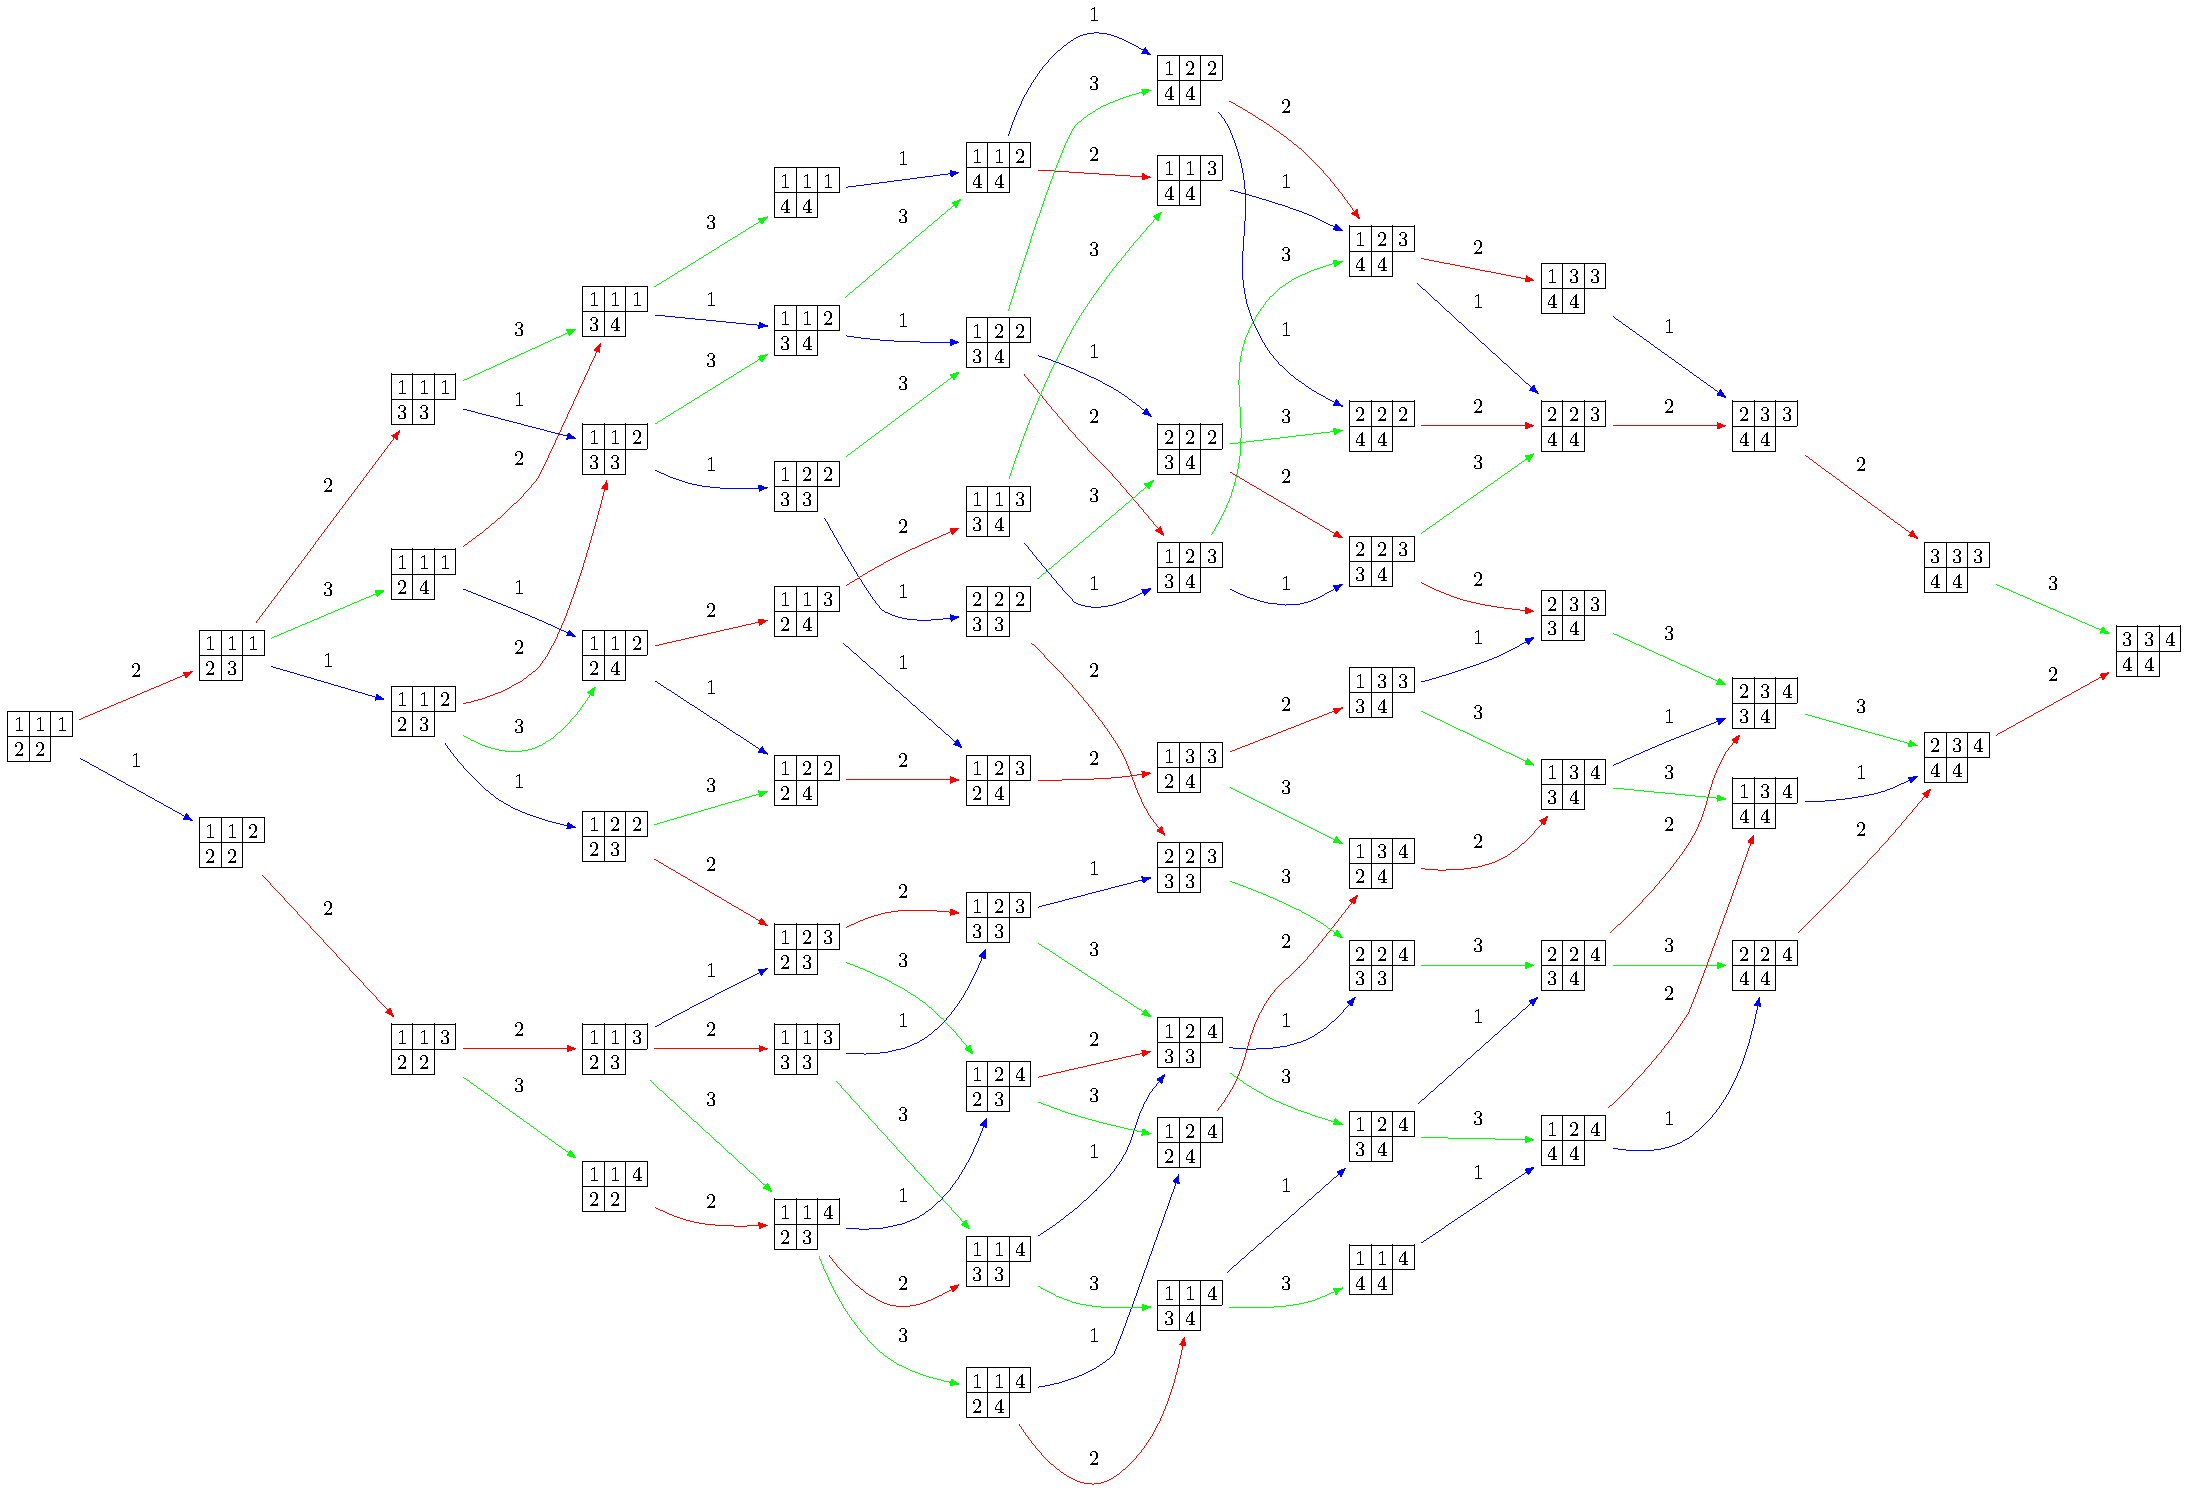
\includegraphics[width=.95\columnwidth]{Pictures/crystal-A3-32}}
\end{frame}

\begin{frame}{\fr{Objets géométriques}\en{Geometric objects}}
  \centerline{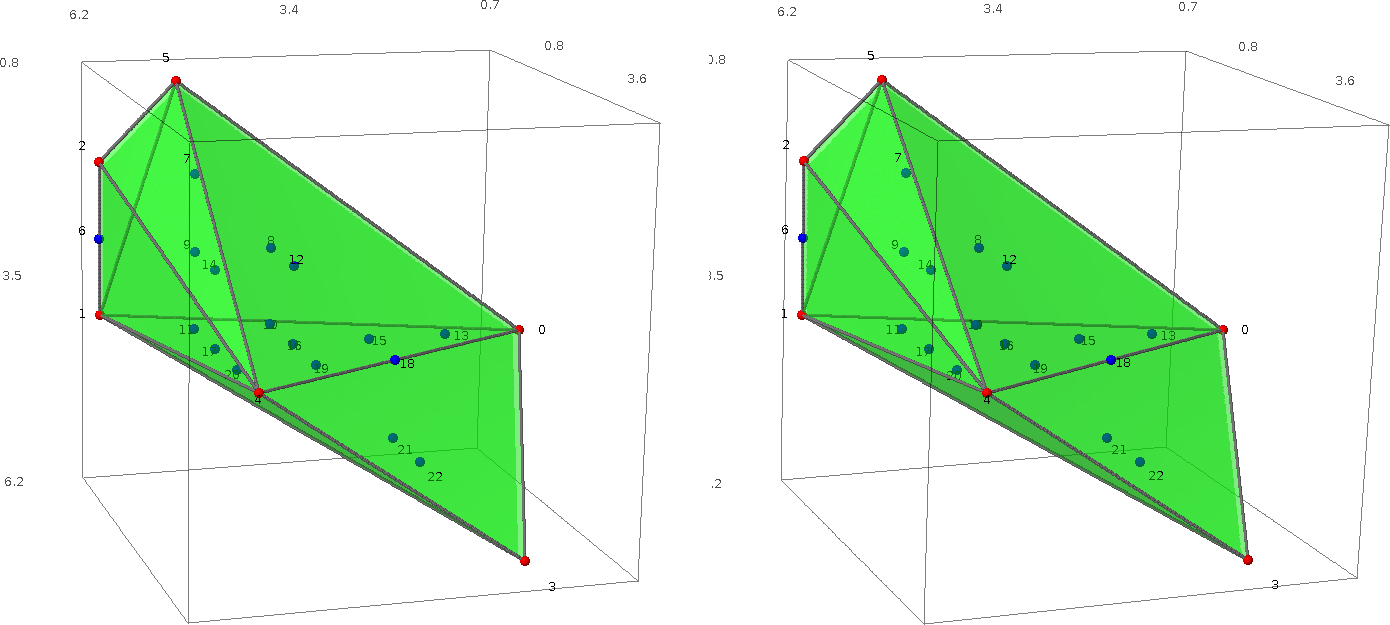
\includegraphics[height=.4\textheight]{Pictures/polytope.png}}

  \centerline{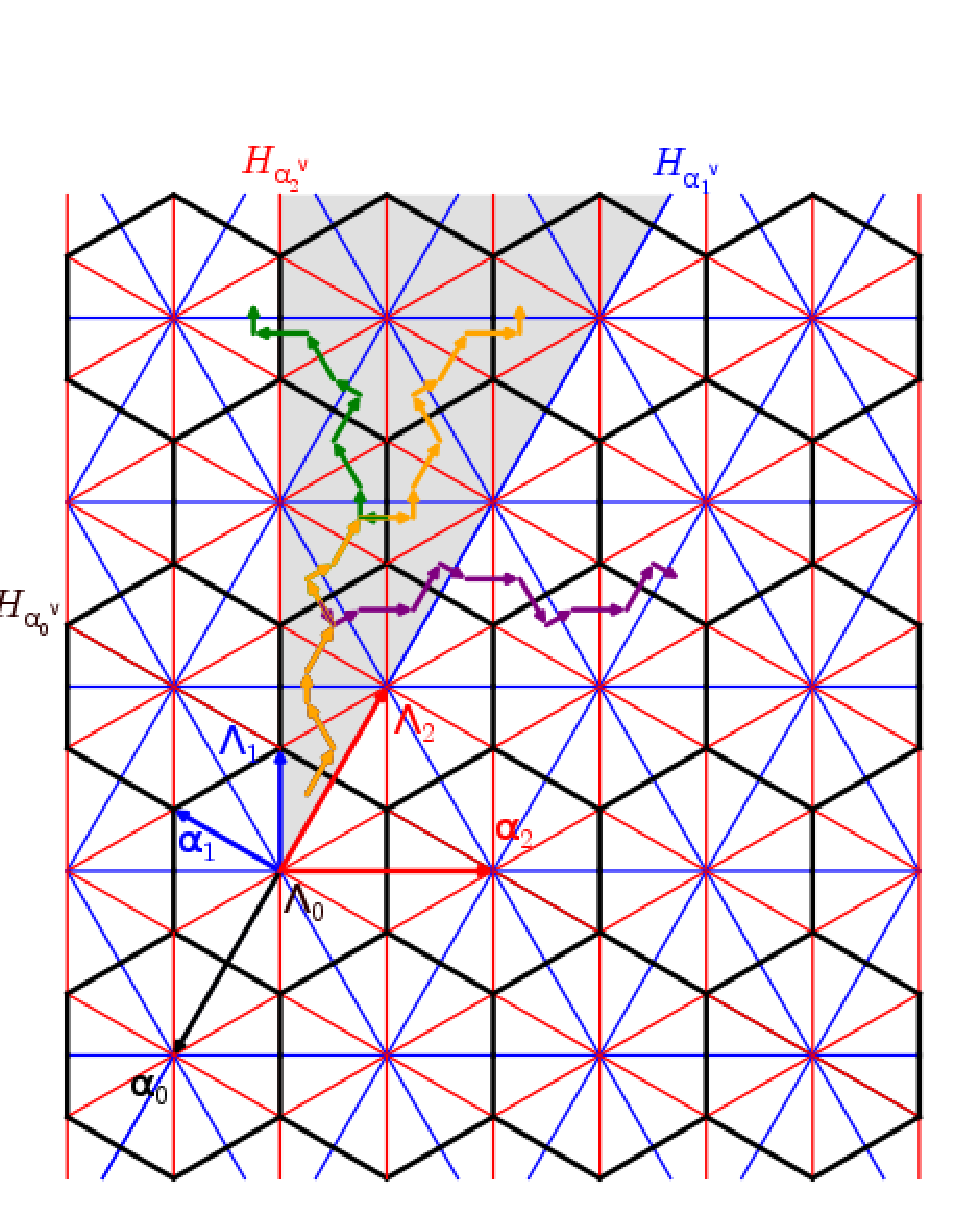
\includegraphics[height=.45\textheight]{Pictures/G2-alcove-path}\qquad
    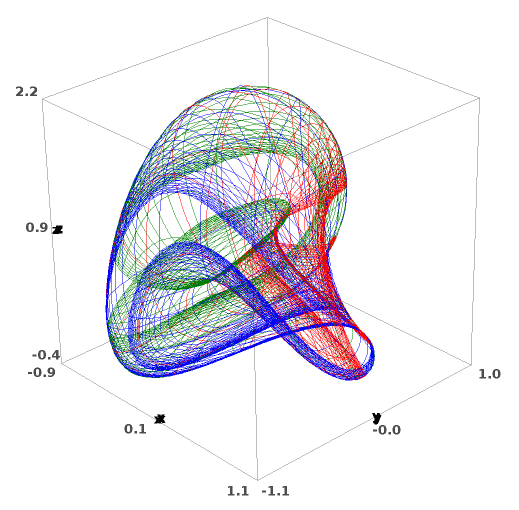
\includegraphics[height=.45\textheight]{Pictures/manifold.png}}
\end{frame}

\begin{frame}{A specific challenge: a rich hierarchy of concepts}

  \begin{bigcenter}
    \only<1>{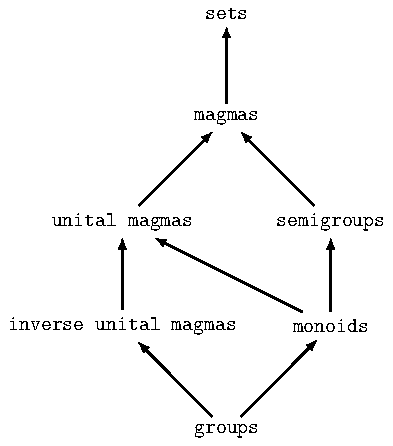
\includegraphics[height=.6\textwidth]{Pictures/Groups-category-graph.pdf}}
    \only<2>{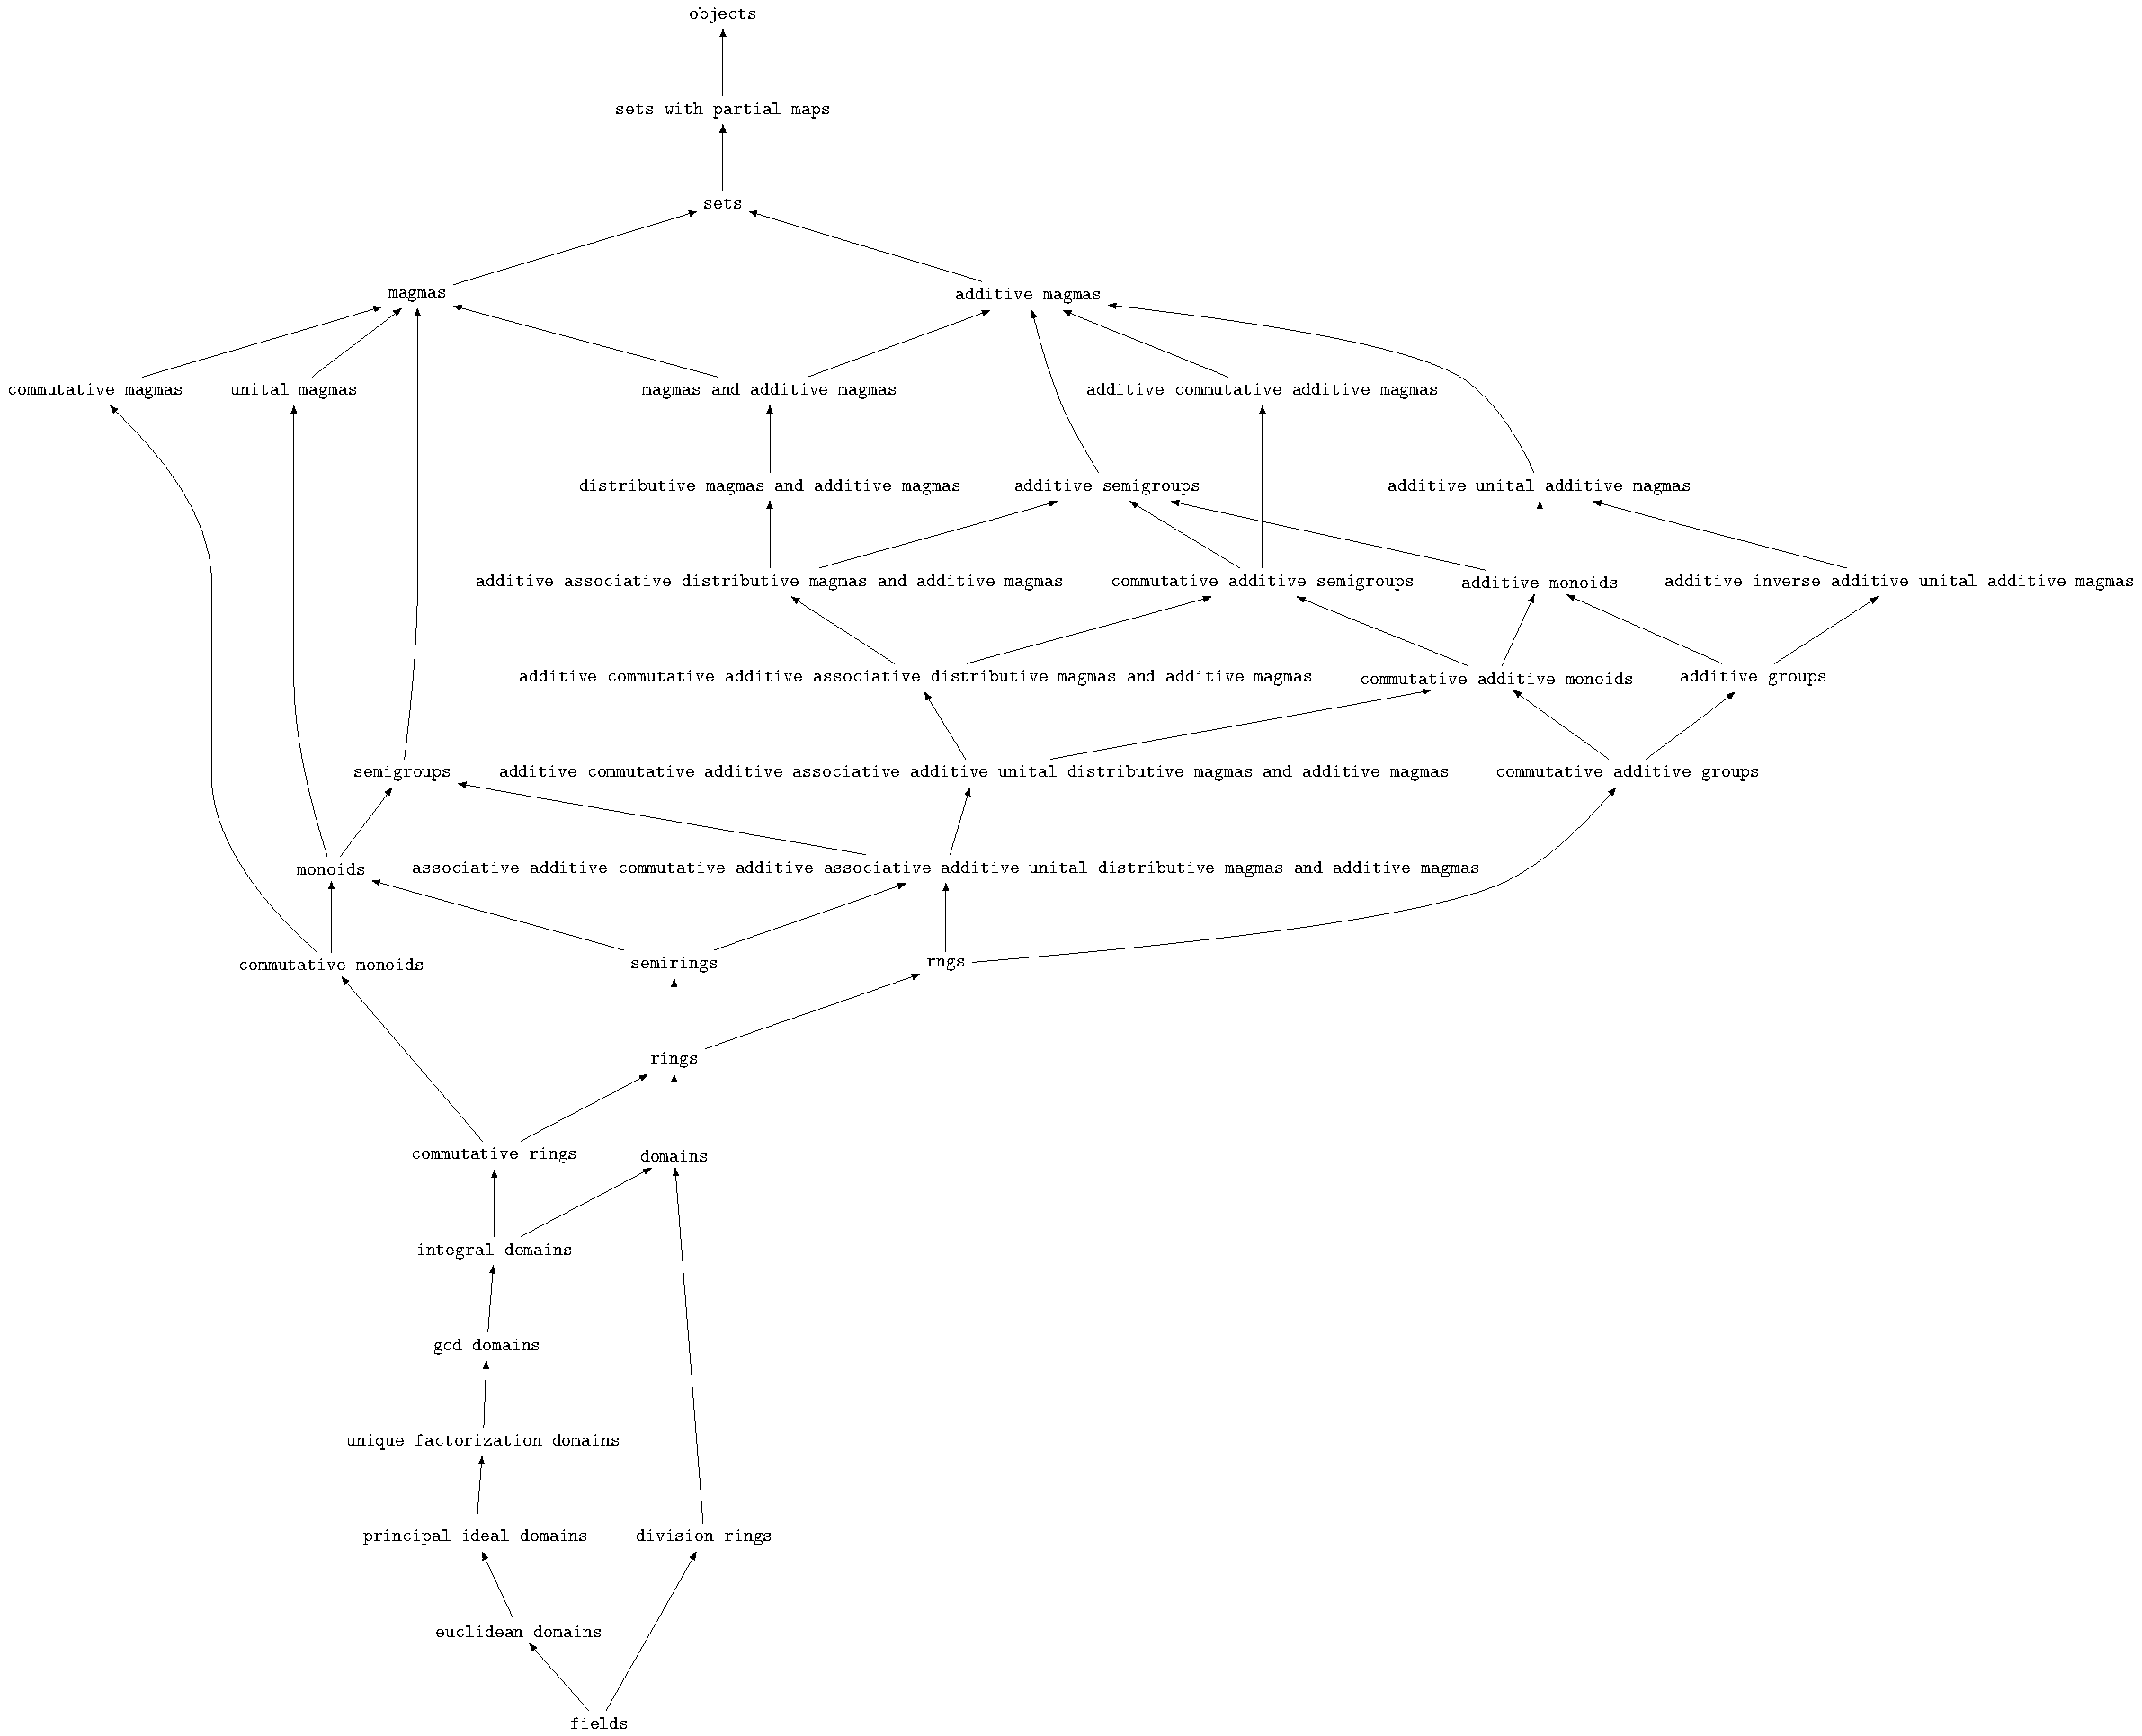
\includegraphics[height=.6\textwidth]{Pictures/Fields-category-graph.pdf}}
    \only<3->{
\includegraphics[width=1.2\textwidth]{Pictures/sage-category-graph.pdf}}
  \end{bigcenter}
  \vfill
\end{frame}

\begin{frame}{What has happened since last review}
  \begin{itemize}
  \item We were able to recruit high profile people
  \item Most technologies we have bet upon (Jupyter, containers, ...)
    have blossomed; \pause\bigskip
  \item VREs based on our toolkit are being deployed at all scales
    (e.g. EGI)
    \pause\bigskip
  \item The toolkit approach is proving its value: impact and adoption
    \pause\bigskip
  \item We reached, trained, and got feedback from many users
    \pause\bigskip
  \end{itemize}

  Risks mitigation!
  
  % By the way: all the points above correspond to risks we had
    % anticipated; they have not materialized, or when they did, our
    % mitigation measures worked
  \begin{item}
  \item Lack of predictability for tasks that are pursued jointly
    with the community
  \item Recruitment of high profile staff (competition from industry!)\\
    Project admin situation
    % Our project admin Benoît left us last August for a better paid
    % and more stable situation in the industry; despite three hiring
    % rounds since April, we still do not have a new project Admin.
  \end{itemize}
\end{frame}


% Viviane was invited to deliver keynote Talk about Science and Open
% Source at PyCon
\end{document}

